\documentclass[a4,12pt]{article}
\usepackage[utf8]{inputenc}
\usepackage[spanish]{babel}
\usepackage[margin=3cm]{geometry}
\usepackage{graphicx}
\usepackage{import}
\usepackage{color}
\usepackage{listings}
\usepackage{hyperref}

%\usepackage{times}

\renewcommand{\familydefault}{\sfdefault}


\usepackage{hyperref}

\hypersetup{
    pdfborder = {0 0 0}
}

\title{Trabajo para el departamento de DIS \newline
\LaTeX, GIT y Octave}

\author{Óscar Berrocal Fráhija}



\begin{document}

\maketitle



\begin{abstract}
Este documento tratará de desarrollar un pequeño trabajo en GNU Octave, documentándolo en latex y usando git como repositorio. En paticular, evaluaré el rendimiento de un algoritmo sencillo sobre matrices, que se corresponde a la parte matemática de uno de los efectos cláscios de la demoscene.
\end{abstract}
\newpage
\tableofcontents

\listoffigures

\newpage

\section{Introducción}
La demoscene es una subcultura del arte por ordenador que se especializa en la producción de demos, que son presentaciones audiovisuales con gráficos y sonido generados en tiempo real por el ordenador.
\newline
\newline
Antes del auge de los IBM PC, los ordenadores personales contaban con un hardware poco variado y configurable, existiendo unas limitaciones y características bien conocidas. Grupos de crackers y artistas gráficos por igual trataban de producir toda clase de efectos gráficos y sonoros llevando al límite las capacidades del hardware existente, superando en sus intros con creces lo que grandes compañías de videojuegos eran capaces de producir.
\newline
\newline
\begin{figure}[h!]
  \centering
    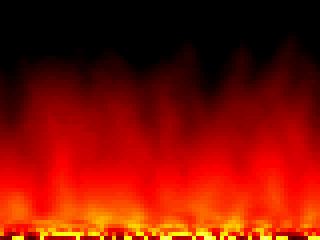
\includegraphics{img/fire}
  \caption{Aspecto del efecto clásico de fuego}
\end{figure}
En la época en que ordenadores tales como el commodore 64, Amiga o Amstrad CPC copaban el mercado, las limitaciones conocidas del hardware permitían implementar de forma precisa este tipo de efectos, creándose un catálogo de conocidos efectos clásicos de la demoscene, como fuego, plasma, túneles, y deformaciones basadas en funciones trigonométricas.
\newline
\newline
\begin{figure}[h!]
  \centering
    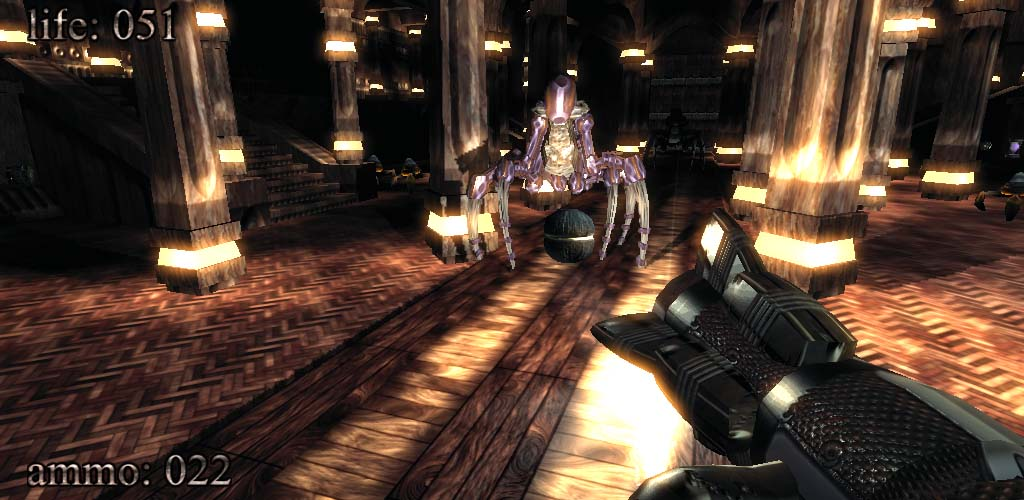
\includegraphics[scale=0.35]{img/kkrieger}
  \caption{.kkrieger, juego completo generado proceduralmente en 96KB}
\end{figure}
Posteriormente, cuando los PC compatibles se asentaron y su hardware fue diversificándose y siendo cada vez más potente, estas restricciones fueron desapareciendo, y en su lugar se trató de generar presentaciones procedurales lo más avanzadas posible tratando de mantener restricciones artificialmente, por ejemplo en el tamaño máximo de los ejecutables.
\newline
\newline
Un ejemplo de ello sería kkrieger, desarrollado por el grupo .theprodukt en 2004, que consigue implementar un juego completo de acción en primera persona en tan sólo 96KB, generando en tiempo real modelos, texturas, niveles y sonido.


\begin{figure}[h!]
  \centering
    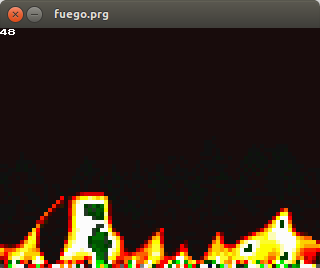
\includegraphics{img/fuego}
  \caption{Otra implementación del mismo efecto, sin buffer}
\end{figure}


\subsection{El efecto de fuego}
De entre los efectos disponibles, he elegido uno relativamente sencillo y fácil de medir. El efecto de fuego que puede verse en la figura 1, trabaja sobre una matiz, haciendo operaciones matemáticas sencillas. En los primeros PCs compatibles, era muy común el modo 13 de vídeo, que ofrecía una resolución de 320x200 pixel y 8 bits de profundidad de color (256 colores). Ajustando dicha paleta de colores a un degradado de tonos de rojos, naranjas y amarillos, de más oscuro a más claro (siendo el cero el negro, y el 255 el color más brillante), podemos definir una matriz de 320x200 bytes, cuyas posiciones se corresponden con píxeles de pantalla en el modo de vídeo, y el valor de cada posición con el color que se muestra en dicha posición.
\newline
\newline
En cada fotograma, la fila inferior de la matriz (o pantalla) se rellena de números aleatorios, y se hace un recorrido al resto de la matriz, calculando su valor como el promedio entre los puntos colindantes:\newline
[tex]punto[x,y] = (punto[x-1,y] + punto[x+1,y] + punto[x,y-1] + punto[x,y+1]) / 4;[/tex] \newline
Se trata realmente de un filtro de suavizado de imagen, tomando como imagen el fotograma anterior y una fila inferior de números aleatorios (que sería la fuente de las llamas).
\newline
\newline
El alcance de este trabajo no es la implementación de una intro funcional, sino de la simulación en octave de los cálculos realizados por el efecto en cuestión para distintos tamaños de problema (cálculo en distintos tamaños de matriz), con el fin de comprobar si es posible obtener una tasa aceptable de fotogramas por segundo.

\section{Desarrollo}

El bucle principal del algoritmo en cuestión es el siguiente:
\bigskip
\lstset{language=Octave}
\begin{lstlisting}[frame=single][language=octave]
for n=1:width-1
	A(height-1, n) = rand();
endfor

for i=2:height-2
 for j=2:width-2
  A(i, j) = (A(i-1,j) + A(i+1,j) + A(i,j-1) + A(i,j+1) ) / 4;
 endfor
endfor
\end{lstlisting}

Se parte de una matriz de dimensiones \(width*height\) (\(height*width\) en representación de octave, para permitir dibujarlo en pantalla directamente), inicialmente con todas sus posiciones a cero. En cada iteración del bucle, la línea base se llena de números aleatorios (en este caso, entre 0 y 1, para ser dibujados correctamente por octave. En el caso del modo 13 de VGA, serían valores entre 0 y 255).
\newline
\newline
Finalmente se hace una media, para cada pixel, de los 4 píxeles colindantes. Se trata de un efecto de desenfoque sencillo, del que puede haber multitud de variantes. Podemos simular unos cuantos fotogramas y proceder a dibujar una imagen:
\bigskip
\lstset{language=Octave}
\begin{lstlisting}[frame=single][language=octave]
width = 40;
height = 30;
A = zeros(height, width);

tic;
for it = 1:150
  for n=1:width-1
    A(height-1, n) = rand();
  endfor

  for i=2:height-2
    for j=2:width-2
      A(i,j) = (A(i-1,j)+A(i+1,j)+A(i,j-1)+A(i,j+1))/4;
    endfor
  endfor
endfor
toc;
imshow(A);
\end{lstlisting}

Se ha elegido un tamaño muy pequeño del problema para obtener un resultado rápido. La figura 4 muestra el resultado de esta ejecución.
\begin{figure}[h!]
  \centering
    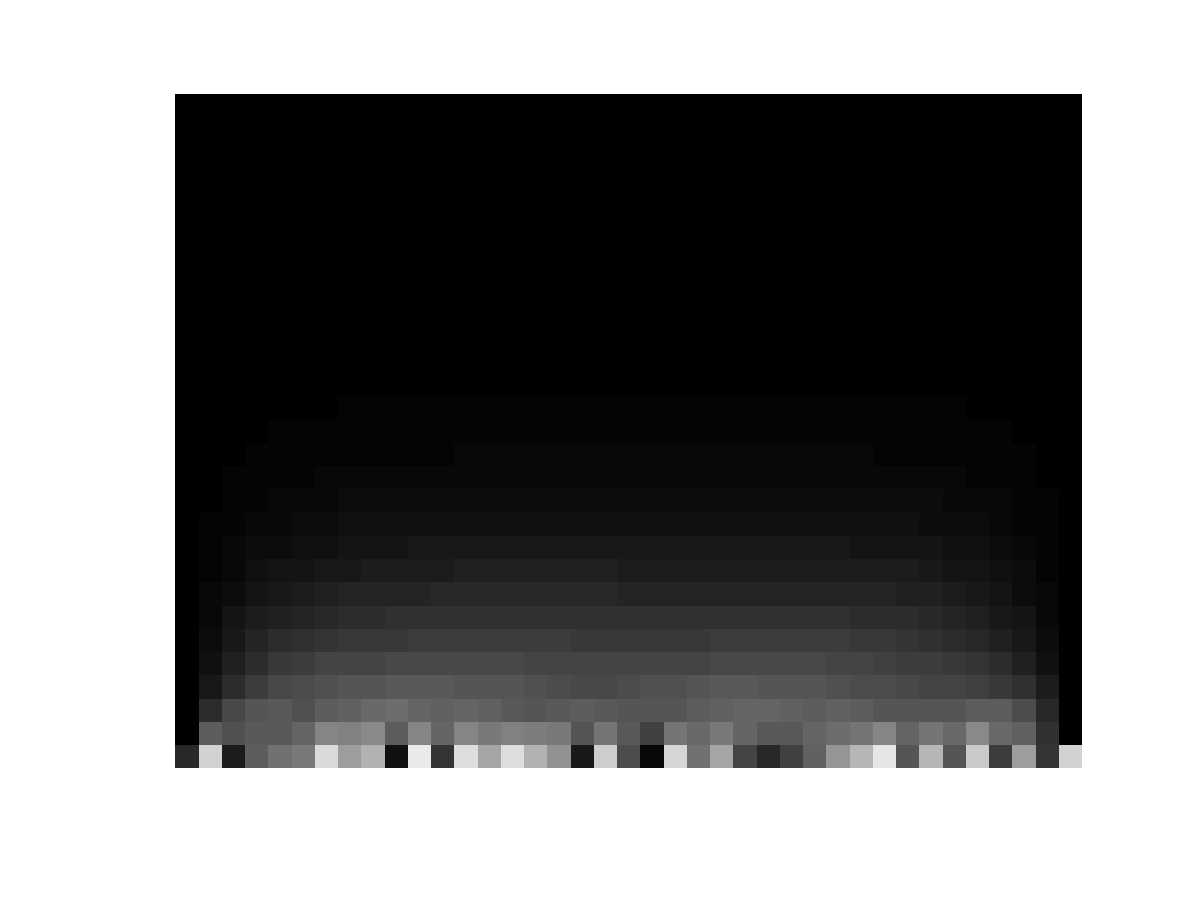
\includegraphics[scale=1.25]{img/resultado}
  \caption{Resultado obtenido en la ejecución en octave tras 150 iteraciones}
\end{figure}

\subsection{Estudio de tiempo de ejecución: consideraciones previas}

Hay una serie de consideraciones que no podemos obviar respecto al rendimiento del algoritmo, que hacen que Octave/Matlab no sea el lenguaje más adecuado para la ejecución de este tipo de efectos:

\begin{itemize}
\item En primer lugar, estamos trabajando con operaciones de punto flotante. De acuerdo con la documentación de intel, en la mayor parte de sus procesadores podemos asumir un ciclo de ejecución para operaciones aritméticas de enteros y 5 ciclos para operaciones flotantes.\cite{intelLatency} Aunque en realidad intervienen muchos factores (como aciertos de caché, paralelismo, u otros procesos en ejecución), podemos asumir que el hecho de no trabajar con enteros hará que el algoritmo sea, inicialmente, como mínimo cinco veces más lento.
\item Por otro lado, no estamos trabajando con punteros. La reserva de memoria contigua y accesos mediante aritmética de punteros nos permiten aumentar sustancialmente los aciertos en caché, mejorando el tiempo de ejecución.
\item Del mismo modo, los desplazamientos de bits permiten agilizar las operaciones de división por números potencia de dos como es el caso.
\end{itemize}

Estos son los factores previsibles que tendrán un gran impacto en el rendimiento de la aplicación. Simplificando mucho, podemos darnos por satisfechos si el tiempo de ejecución es tan sólo cinco veces mayor del esperado en la misma implementación en C (donde esperamos un mínimo de 25 imágenes por segundo a una resolución de 320x240 pixels)

\subsection{Estudio empírico del tiempo de ejecución}

Para medir el rendimiento, vamos a ejecutar el algoritmo con distintos tamaños de matriz, con 100 iteraciones por cada ejecución, y haremos una media de los tiempos de ejecución para cada tamaño del problema.
\newline
\newline
La ejecuión del equivalente en C debe ofrecer un mínimo de 25 fotogramas por segundo. Eso significa que el tiempo de ejecución de cada iteración debería ser de \(1/25\) segundos para obtener tal rendimiento.

\subsubsection{Estudio empírico del tiempo de ejecución}

Se va a ejecutar 100 iteraciones del algoritmo para las resoliciones de pantalla de la siguiente tabla:\\
\begin{tabular}{ | r | l |}
\hline
  Resolución & Tiempo \\
\hline
  40x30 & - \\
  80x60 & - \\
  120x80 & - \\
  320x200 & - \\
  640x480 & - \\
\hline
\end{tabular}

Para cada resolución, se guardará el tiempo de ejecución de sus 100 iteraciones, 6y se calculará el tiempo promedio por fotograma dividiendo el resultado entre cien.
\\
\\
El programa final para las pruebas queda como sigue:
\bigskip
\lstset{language=Octave}
\begin{lstlisting}[frame=single][language=octave]
global h;
global w;

function res = calcularFuego( w, h )
 res = 0;
 height = h;
 width = w;
 A = zeros(height, width);

 tic;
 for it = 1:100
  for n=1:width-1
	A(height-1, n) = rand();
  endfor
  for i=2:height-2
   for j=2:width-2
	A(i,j) = (A(i-1,j)+A(i+1,j)+A(i,j-1)+A(i,j+1))/4;
    endfor
  endfor
endfor
res = toc;
endfunction

tiempos(1) = calcularFuego(40, 30);
tiempos(2) = calcularFuego(80, 60);
tiempos(3) = calcularFuego(120, 80);
tiempos(4) = calcularFuego(160, 120);
tiempos(5) = calcularFuego(320, 200);
tiempos(6) = calcularFuego(640, 480);

barh(tiempos);
title('Tiempos de ejecucion para tam. de problema');
saveas (1, "tiempos.png");
tiempos
\end{lstlisting}
sdafsdgsd

\begin{thebibliography}{99}
\bibitem{intelLatency} Instruction Latencies in Assembly Code for 64-Bit Intel® Architecture:\\ \url{https://software.intel.com/en-us/articles/instruction-latencies-in-assembly-code-for-64-bit-intel-architecture?language=en}
\bibitem{inlineequations} In-line equations:\\ \url{http://www.math.tamu.edu/~boas/courses/math696/LaTeX-in-line-equations.html}
\end{thebibliography}
\end{document}

